%compare accuracy of the algorithms
%put global feature importance for each algorithm and compare them
%for the best algorithm, put feature importance for each region and compare them


\chapter{Results}

\section{Results of the Models}

\begin{table}[htbp]
    \centering
    \begin{tabular}{|l|c|c|}
    \hline
    \textbf{Model}           & \textbf{Accuracy} & \textbf{Weighted Average of Precision} \\ \hline
    Logistic Regression & 85.42\%          & 0.73                \\ \hline
    Decision Tree       & 68.64\%          & 0.78              \\ \hline
    Random Forest      & 83.02\%          & 0.83             \\ \hline
    Naïve Bayes         & 53.52\%          & 0.54               \\ \hline
    KNN                 & 80.73\%          & 0.84               \\ \hline
    \end{tabular}
    \caption{Accuracy and Weighted Average of Precision of Different Models}
    \end{table}
    
According to the results shown in the table above, the model with the highest accuracy is Logistic Regression with 85.42\%, but this is due to the high imbalance of the dataset, so it's not considered the best model.\\
Random Forest has the higher value of accuracy among the other models, and it also has the highest weighted average of precision. Furthermore, its confusion matrix has the highest number of correct predictions. This makes Random Forests the best model for this dataset with 83.02\% accuracy. \\
Another pretty good result was obtained by KNN, with an accuracy of 80.73\% and a weighted average of precision of 0.84.\\
In general, all the models have high accuracy values, which indicates that the dataset is well-suited for classification. Even the worst model, Naïve Bayes, has an accuracy of 53.52\%, which is not bad.\\
Furthermore, our accuracy results are better than the article studied for the literature, in which the best algorithm, Logistic Regression, had an accuracy of 52\%. This could be due to the fact that their dataset was smaller and less diverse than the dataset used in this study.
\\

\newpage

\section{Global Feature Importance Analysis}

It's important to understand the global importance of the features in the dataset to be able to make better predictions.

The feature importance is extracted from the Random Forest model, which is the best model for this dataset.

The Random Forest model shows that globally many features are important for predicting the popularity of a song: \textit{acousticness} is the most important, but also \textit{speechiness}, \textit{valence}, \textit{duration}, \textit{tempo}, \textit{instrumentalness}, \textit{liveness}, \textit{danceability}, \textit{energy} and \textit{loudness} have similarly high values of importance. The least important features are \textit{key}, \textit{mode} and \textit{time signature}. These last two features were already shown to not be important in the correlation matrix.

On the other hand, all the other models show that 
\textit{dancebility} is the most important feature, with a significant difference from the other features.

This difference can be attributed to the inherent complexity and flexibility of the Random Forest
algorithm, which allows it to capture intricate patterns and interactions in the data that other models may not.\\
Also the literature supports the \textit{danceability} as the most important feature for predicting the popularity of a song, with a significant difference from the other features.\\



\textbf{Global Feature Importance}

\begin{figure} [H]
    \centering
    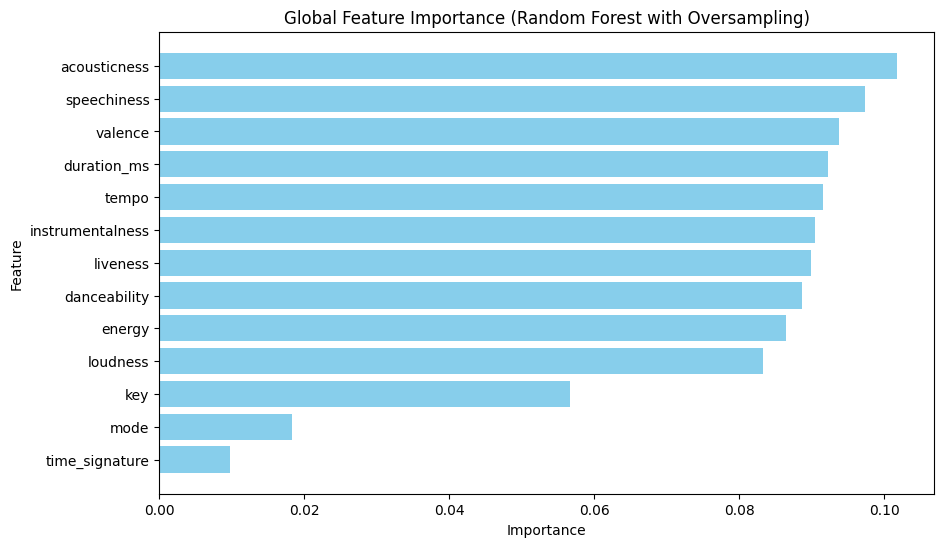
\includegraphics[width=0.8\textwidth]{media/random_forest_feature_imp_global.png}
    \caption{Global Feature Importance Using Random Forests Model}
    \label{fig:feature_importance}
\end{figure}

\newpage

\section{Regional Feature Importance Analysis}


The feature importance is extracted not only globally but also for each region. To do that we decide to consider the Random Forest model as the best model.
This analysis helps to understand how the music tastes of different regions are shaped by audio features.
The most important features for each region are shown below. The mean values of these features are also given to help understand the music tastes of each region.

%NB: These graphs also show the region column, it's a waste of space, we should remove it

\subsection{Feature Importance for Each Region Extracted From Random Forest Model}
\begin{figure}[h]
    \centering
    \begin{minipage}{0.45\textwidth}
        \centering
        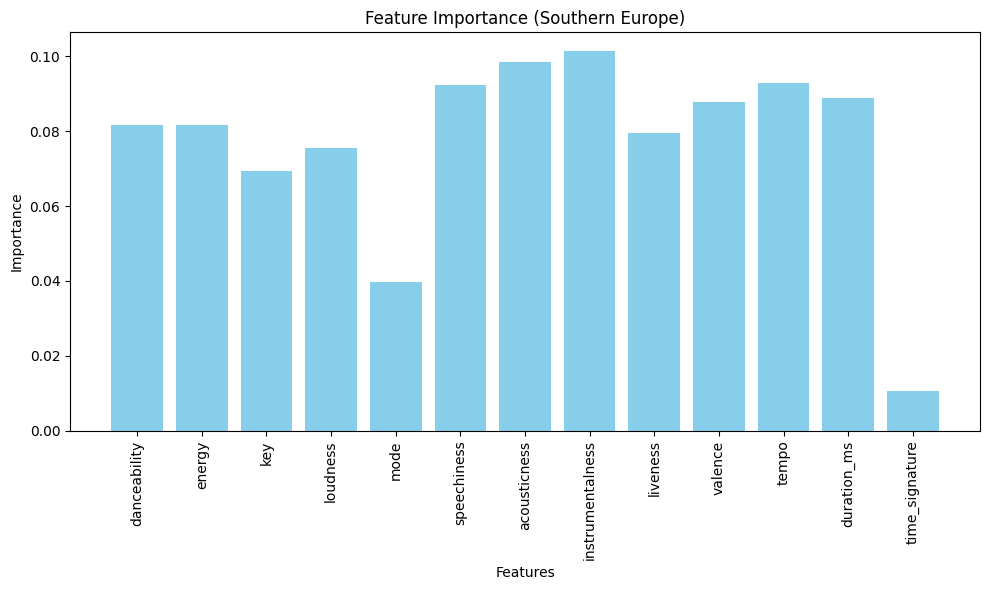
\includegraphics[width=\linewidth]{media/rf_feature_imp_northen_europe.png}
        \caption{Feature Importance in North Europe}
    \end{minipage}%
    \hspace{0.05\textwidth} % Space between the two figures
    \begin{minipage}{0.45\textwidth}
        \centering
        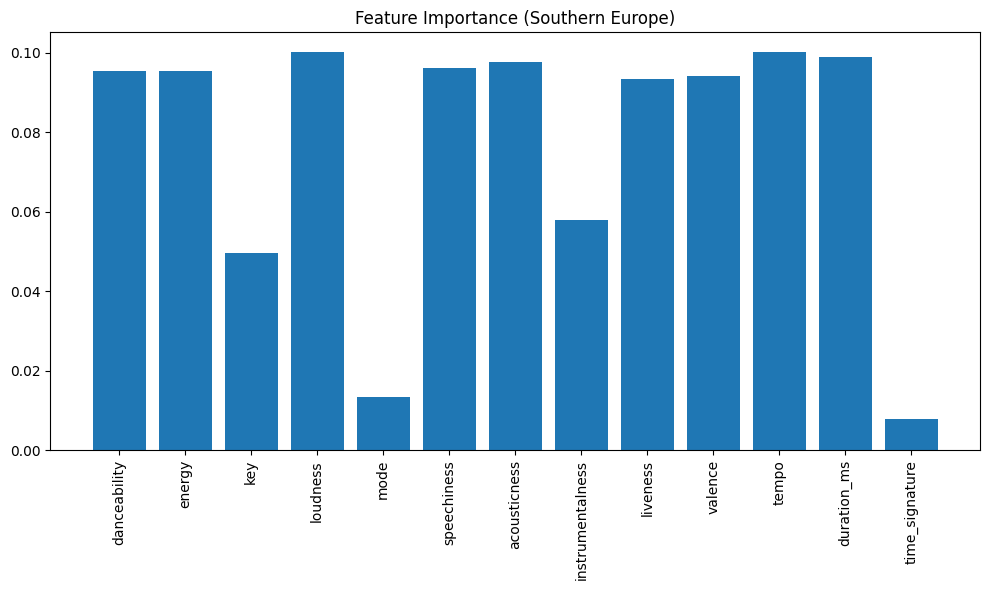
\includegraphics[width=\linewidth]{media/rf_feature_imp_southern_europe.png}
        \caption{Feature Importance in South Europe}
    \end{minipage}
\end{figure}
\begin{figure}[h]
    \centering
    \begin{minipage}{0.45\textwidth}
        \centering
        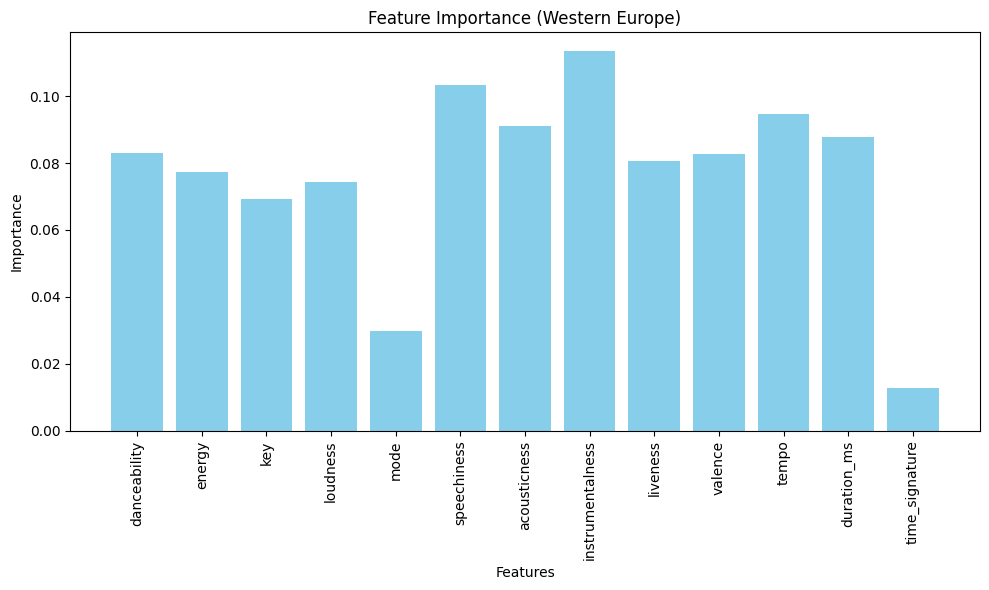
\includegraphics[width=\linewidth]{media/rf_feature_imp_western_europe.png}
        \caption{Feature Importance in Western Europe}
    \end{minipage}%
    \hspace{0.05\textwidth} % Space between the two figures
    \begin{minipage}{0.45\textwidth}
        \centering
        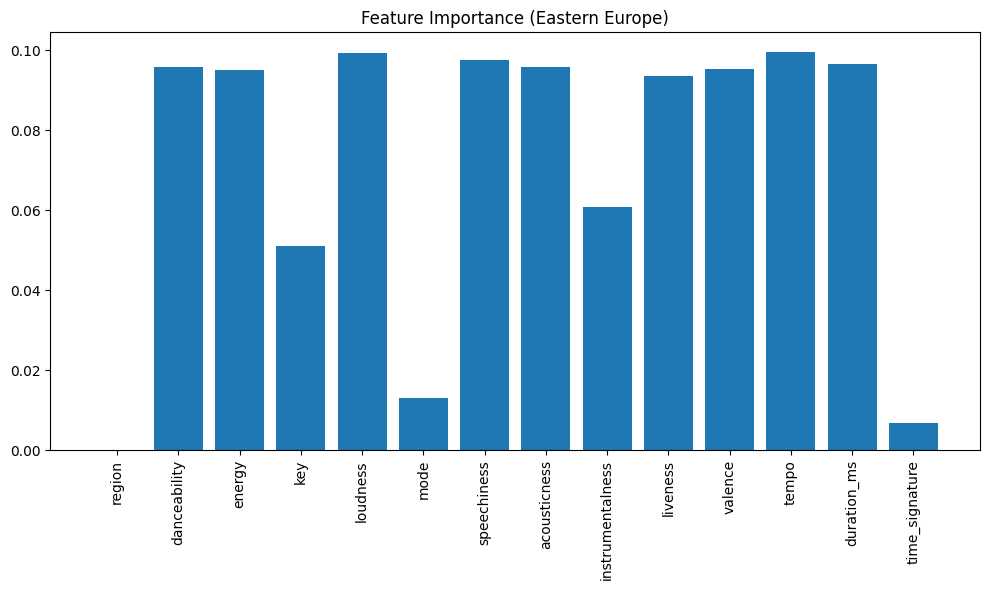
\includegraphics[width=\linewidth]{media/rf_feature_imp_eastern_europe.png}
        \caption{Feature Importance in Eastern Europe}
    \end{minipage}
\end{figure}
\begin{figure}[h]
    \centering
    \begin{minipage}{0.45\textwidth}
        \centering
        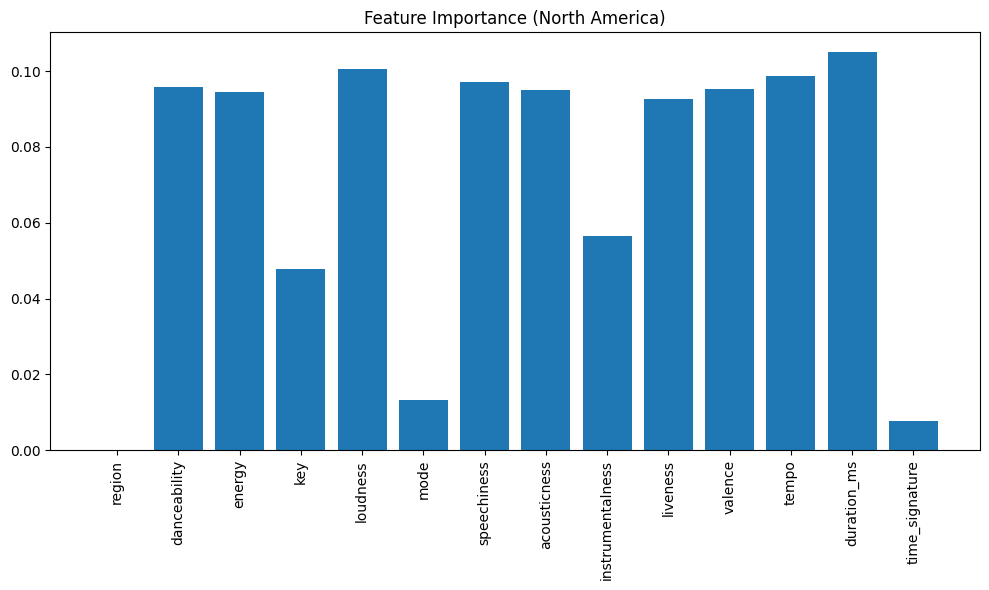
\includegraphics[width=\linewidth]{media/rf_feature_imp_north_america.png}
        \caption{Feature Importance in North America}
    \end{minipage}%
    \hspace{0.05\textwidth} % Space between the two figures
    \begin{minipage}{0.45\textwidth}
        \centering
        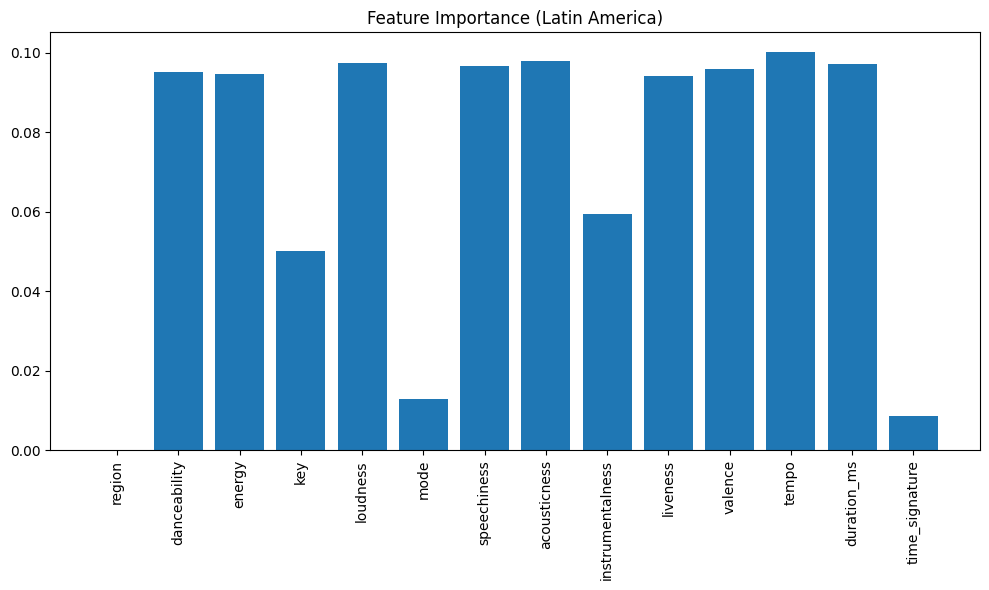
\includegraphics[width=\linewidth]{media/rf_feature_imp_latin_america.png}
        \caption{Feature Importance in Latin America}
    \end{minipage}
\end{figure}
\begin{figure}[h]
    \centering
    \begin{minipage}{0.45\textwidth}
        \centering
        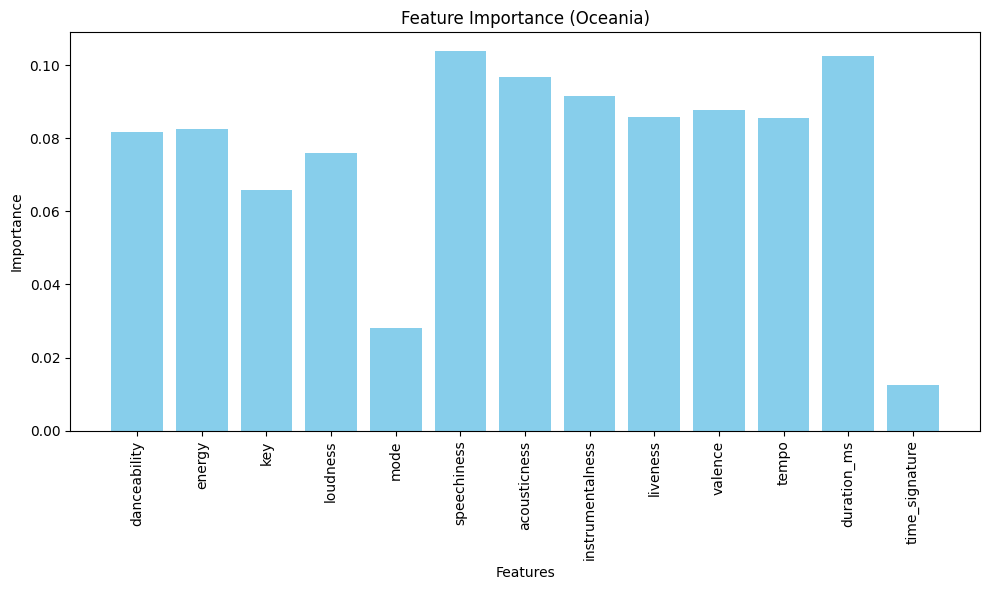
\includegraphics[width=\linewidth]{media/rf_feature_imp_ocenia.png}
        \caption{Feature Importance in Oceania}
    \end{minipage}%
    \hspace{0.05\textwidth} % Space between the two figures
    \begin{minipage}{0.45\textwidth}
        \centering
        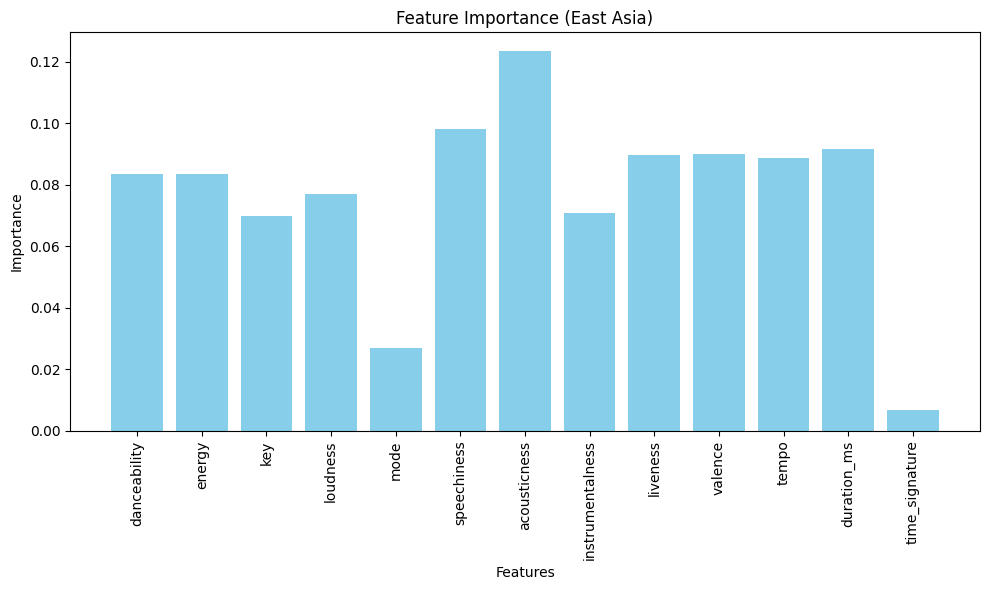
\includegraphics[width=\linewidth]{media/rf_feature_imp_east_asia.png}
        \caption{Feature Importance in East Asia}
    \end{minipage}
\end{figure}
\begin{figure}[h]
    \centering
    \begin{minipage}{0.45\textwidth}
        \centering
        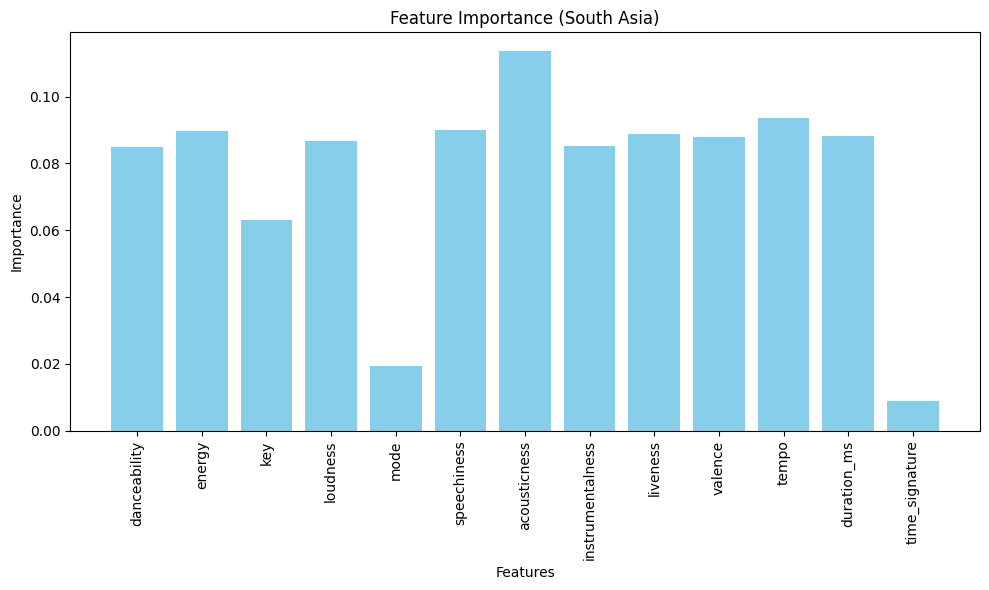
\includegraphics[width=\linewidth]{media/rf_feature_imp_south_asia.png}
        \caption{Feature Importance in South Asia}
    \end{minipage}%
    \hspace{0.05\textwidth} % Space between the two figures
    \begin{minipage}{0.45\textwidth}
        \centering
        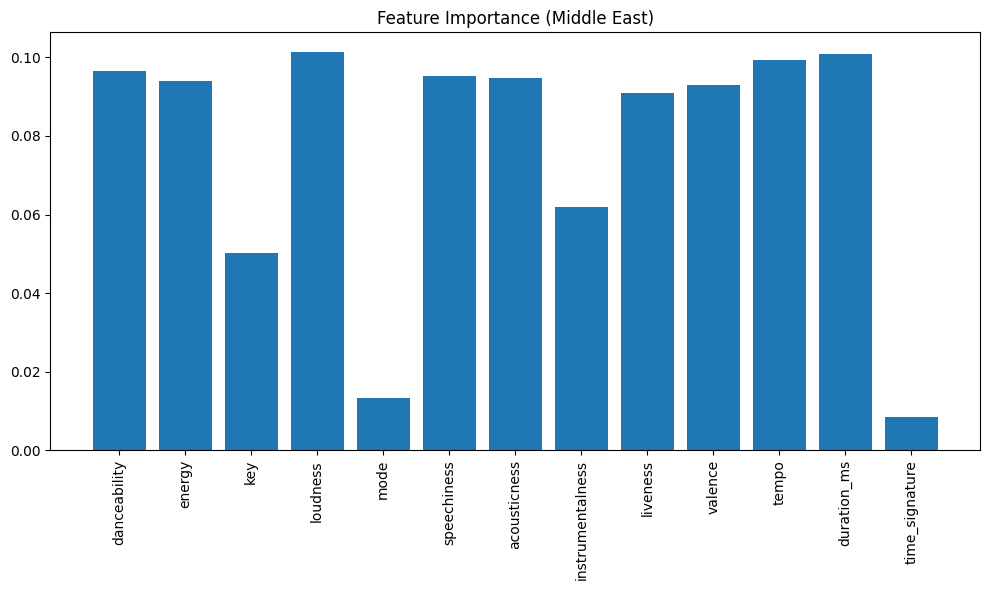
\includegraphics[width=\linewidth]{media/rf_feature_imp_middle_east.png}
        \caption{Feature Importance in Middle East}
    \end{minipage}
\end{figure}
\begin{figure}[h]
    \centering
    \begin{minipage}{0.45\textwidth}
        \centering
        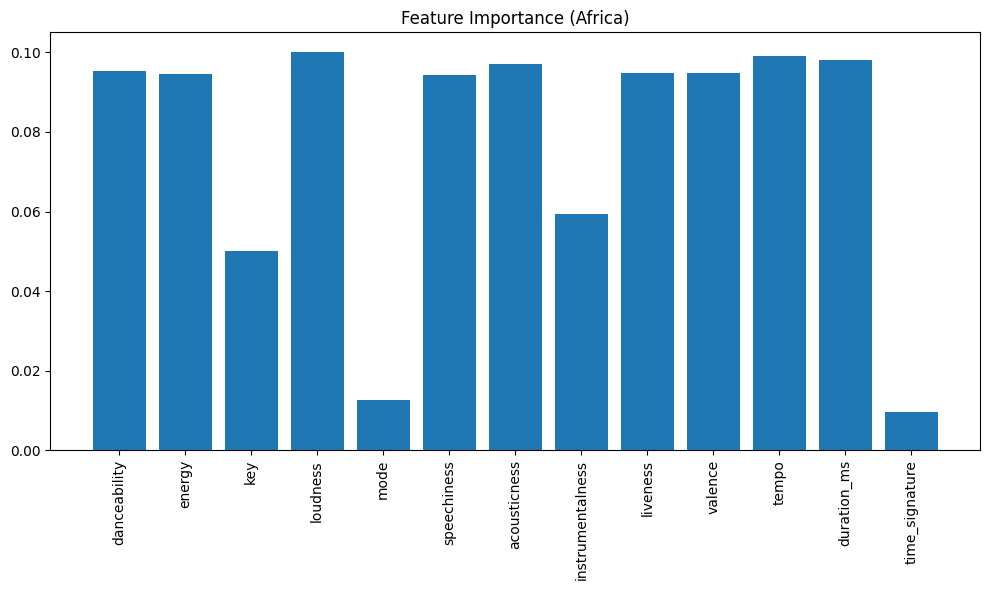
\includegraphics[width=\linewidth]{media/rf_feature_imp_africa.png}
        \caption{Feature Importance in Africa}
    \end{minipage}
\end{figure}

\clearpage 

\subsection{Important Features for Each Region and Their Mean Values}

The different regions tend to have a general coherence in the importance of the features, but there are still differences in the music tastes of each region.\\



\textbf{Northern Europe}
\begin{enumerate}
    \item \textbf{Instrumentalness}: Importance: 0.1073, Mean Value: 0.04
    \item \textbf{Speechiness}: Importance: 0.1005, Mean Value: 0.11
    \item \textbf{Acousticness}: Importance: 0.0994, Mean Value: 0.23
    \item \textbf{Duration\_ms}: Importance: 0.0935, Mean Value: 203514.75
    \item \textbf{Tempo}: Importance: 0.0918, Mean Value: 121.29
\end{enumerate}

\textbf{Southern Europe}
\begin{enumerate}
    \item \textbf{Instrumentalness}: Importance: 0.1007, Mean Value: 0.04
    \item \textbf{Acousticness}: Importance: 0.0980, Mean Value: 0.27
    \item \textbf{Speechiness}: Importance: 0.0933, Mean Value: 0.12
    \item \textbf{Tempo}: Importance: 0.0929, Mean Value: 121.24
    \item \textbf{Duration\_ms}: Importance: 0.0886, Mean Value: 210862.34
\end{enumerate}

\textbf{Western Europe}
\begin{enumerate}
    \item \textbf{Instrumentalness}: Importance: 0.1137, Mean Value: 0.06
    \item \textbf{Speechiness}: Importance: 0.1029, Mean Value: 0.15
    \item \textbf{Tempo}: Importance: 0.0946, Mean Value: 120.90
    \item \textbf{Acousticness}: Importance: 0.0909, Mean Value: 0.25
    \item \textbf{Duration\_ms}: Importance: 0.0873, Mean Value: 205864.40
\end{enumerate}

\textbf{Eastern Europe}
\begin{enumerate}
    \item \textbf{Speechiness}: Importance: 0.1009, Mean Value: 0.13
    \item \textbf{Acousticness}: Importance: 0.0973, Mean Value: 0.24
    \item \textbf{Instrumentalness}: Importance: 0.0967, Mean Value: 0.06
    \item \textbf{Tempo}: Importance: 0.0928, Mean Value: 122.33
    \item \textbf{Valence}: Importance: 0.0872, Mean Value: 0.47
\end{enumerate}

\textbf{North America}
\begin{enumerate}
    \item \textbf{Acousticness}: Importance: 0.1013, Mean Value: 0.24
    \item \textbf{Duration\_ms}: Importance: 0.0993, Mean Value: 206987.98
    \item \textbf{Speechiness}: Importance: 0.0950, Mean Value: 0.13
    \item \textbf{Valence}: Importance: 0.0914, Mean Value: 0.46
    \item \textbf{Tempo}: Importance: 0.0898, Mean Value: 121.36
\end{enumerate}


\textbf{Latin America}
\begin{enumerate}
    \item \textbf{Tempo}: Importance: 0.0980, Mean Value: 122.61
    \item \textbf{Speechiness}: Importance: 0.0971, Mean Value: 0.11
    \item \textbf{Valence}: Importance: 0.0956, Mean Value: 0.58
    \item \textbf{Acousticness}: Importance: 0.0953, Mean Value: 0.29
    \item \textbf{Duration\_ms}: Importance: 0.0886, Mean Value: 217127.50
    
\end{enumerate}

\textbf{Oceania}
\begin{enumerate}
    \item \textbf{Speechiness}: Importance: 0.1027, Mean Value: 0.12
    \item \textbf{Duration\_ms}: Importance: 0.1024, Mean Value: 213396.98
    \item \textbf{Acousticness}: Importance: 0.0959, Mean Value: 0.23
    \item \textbf{Instrumentalness}: Importance: 0.0923, Mean Value: 0.05
    \item \textbf{Valence}: Importance: 0.0878, Mean Value: 0.47
    
\end{enumerate}

\textbf{East Asia}
\begin{enumerate}
    \item \textbf{Acousticness}: Importance: 0.1223, Mean Value: 0.30
    \item \textbf{Speechiness}: Importance: 0.0982, Mean Value: 0.08
    \item \textbf{Liveness}: Importance: 0.0910, Mean Value: 0.18
    \item \textbf{Duration\_ms}: Importance: 0.0902, Mean Value: 229571.73
    \item \textbf{Valence}: Importance: 0.0896, Mean Value: 0.47
\end{enumerate}

\textbf{South Asia}
\begin{enumerate}
    \item \textbf{Acousticness}: Importance: 0.1135, Mean Value: 0.36
    \item \textbf{Tempo}: Importance: 0.0928, Mean Value: 119.92
    \item \textbf{Energy}: Importance: 0.0914, Mean Value: 0.58
    \item \textbf{Speechiness}: Importance: 0.0902, Mean Value: 0.08
    \item \textbf{Liveness}: Importance: 0.0885, Mean Value: 0.17
\end{enumerate}


\textbf{Middle East}
\begin{enumerate}
    \item \textbf{Instrumentalness}: Importance: 0.1062, Mean Value: 0.06
    \item \textbf{Acousticness}: Importance: 0.1010, Mean Value: 0.30
    \item \textbf{Duration\_ms}: Importance: 0.0959, Mean Value: 213894.57
    \item \textbf{Speechiness}: Importance: 0.0912, Mean Value: 0.10
    \item \textbf{Valence}: Importance: 0.0894, Mean Value: 0.47
\end{enumerate}


\textbf{Africa}
\begin{enumerate}
    \item \textbf{Instrumentalness}: Importance: 0.1137, Mean Value: 0.06
    \item \textbf{Speechiness}: Importance: 0.1029, Mean Value: 0.15
    \item \textbf{Tempo}: Importance: 0.0946, Mean Value: 120.90
    \item \textbf{Acousticness}: Importance: 0.0909, Mean Value: 0.25
    \item \textbf{Duration\_ms}: Importance: 0.0873, Mean Value: 205864.40
\end{enumerate}

\newpage
\subsection{Interpretation of the Results}

\begin{itemize}

    \item\textbf{Global Coherence}

    \textit{Instrumentalness}, \textit{Speechiness}, \textit{Acousticness}, and \textit{Duration} emerge consistently as top features in nearly every region, though with different relative importance.
These features often relate to how a song conveys mood and rhythm and might align with the universality of music as a form of emotional expression and storytelling.
The wide influence of Western music on pop culture may have contributed to the popularity of these features, as they are core elements in pop, hip-hop, and electronic genres.


\item\textbf{Region-Specific Preferences}

In \textbf{Latin America} \textit{Tempo} and \textit{Valence} are highly important, reflecting Latin music's rhythmic vibrancy and high-energy, uplifting tones (e.g., salsa, reggaeton). Latin American music often emphasizes danceability, aligning with culturally rooted music traditions focused on rhythm and movement.
In \textbf{East Asia} and \textbf{South Asia} {Acousticness} is prioritized, showing a preference for traditional, soft, or acoustic elements. This aligns with the longstanding cultural appreciation for subtle, melodic sounds in classical and popular Asian music.
In the \textbf{Middle East} \textit{Instrumentalness} and \textit{Acousticness} are essential, reflecting the region's rich heritage of instrumental music and acoustic sounds (e.g., oud, ney). This preference is likely influenced by traditional musical forms that emphasize texture and melody over vocal prominence.


\item\textbf{Shared Importance of Instrumentalness}

\textit{Instrumentalness} appears consistently across \textbf{Northern Europe}, \textbf{Southern Europe}, \textbf{Western Europe}, \textbf{Africa}, and the \textbf{Middle East}. This shared importance suggests a cross-regional appreciation for compositions where instrumental texture plays a major role, which could reflect the influence of classical music traditions that are still prominent in these regions.
Additionally, this trend may point to a cultural appreciation for genres like electronic or ambient music, which often rely heavily on instrumentals.


\item\textbf{Tempo as a Key Feature}

\textit{Tempo} is particularly prominent in \textbf{Latin America} and \textbf{Eastern Europe}, regions with strong dance traditions (e.g., cumbia, salsa, and Balkan beats). A faster or more rhythmic tempo may appeal to these audiences due to the cultural significance of danceable music.
In other regions, such as \textbf{North America}, \textit{Tempo} is present but slightly less emphasized, potentially due to the popularity of more varied genres, including slower-tempo hip-hop and R\&B.


\item\textbf{Duration as a Consistent Feature}

\textit{Duration\_ms} holds similar importance across regions like \textbf{North America}, \textbf{Western Europe}, and \textbf{Oceania}, indicating a common preference for song length that aligns with global pop music standards.
Shorter or moderate-length songs, commonly around 3 to 4 minutes, are more favorable in these regions, aligning with the mainstream pop structure popularized by global record labels and radio formats.


\item\textbf{Valence and Mood Preferences}

\textit{Valence}, which measures musical positiveness, is a notable feature in \textbf{Latin America} and \textbf{North America}, suggesting a preference for more “positive” or “happy” songs. This could reflect cultural preferences for upbeat, feel-good music in these regions, where music often accompanies social gatherings.
In \textbf{East Asia}, however, \textit{Valence} is less prominent, potentially indicating a preference for more emotionally complex or even melancholic tones, which is often present in Asian pop and ballads.


\item\textbf{Impact of Globalization}

Regions with high influence from Western pop culture, such as \textbf{North America}, \textbf{Europe}, and \textbf{Oceania}, show a strong alignment in the importance of core features like \textit{Acousticness} and \textit{Speechiness}, likely due to the widespread dissemination of pop, hip-hop, and EDM.
In contrast, regions with strong traditional music influences (e.g., \textbf{Middle East}, \textbf{East Asia}) retain unique feature preferences, such as a stronger emphasis on \textit{Acousticness} and \textit{Instrumentalness}, reflecting a blend of contemporary and traditional music tastes shaped by both global trends and local heritage.

\item\textbf{Underrepresented Features}

\textit{Energy}, \textit{Key}, and \textit{Mode} are not among the top features for most regions, indicating these are less influential in determining a song’s popularity. This suggests that, despite varying genres and tastes, there’s less of a focus on tonal characteristics and more on rhythmic and acoustic qualities across different regions.

\item\textbf{Evolution of Regional Music Preferences}

Over time, these differences in preferences might evolve as global trends influence local tastes, or as
regions increasingly revert to traditional forms in response to external influences. Monitoring how
these values change over time could offer insights into the trajectory of regional music trends. These
considerations highlight the diversity in music preferences across regions, while also emphasizing
certain universal elements that transcend cultural boundaries. Understanding these nuances helps
map out how cultural and social factors influence regional music trends.

\end{itemize}